\subsection{Uso de MLOps mediante despliegue en un ambiente controlado, con la capacidad de monitorear y mejorar continuamente el rendimiento del modelo}

\subsubsection{Despliegue en Cloud}

La plataforma DagsHub se presenta como una solución integral específicamente diseñada para la ingeniería de software, fusionando de manera efectiva las funcionalidades esenciales de control de versiones del código, versionado de datos y seguimiento de experimentos. Este enfoque unificado facilita la administración de proyectos en los campos de aprendizaje automático, desde la fase inicial de experimentación hasta la colaboración en equipo y la entrega de resultados. \newline

La integración de DagsHub con herramientas clave como Git, DVC y MLFlow fortalece aún más su versatilidad. Cada una de estas herramientas desempeña un papel específico y complementario en el proceso. Git se encarga del control de versiones del código, DVC se especializa en la gestión de datos, mientras que MLFlow se enfoca en el seguimiento de experimentos y versionado de modelos. Esta plataforma permite a cada herramienta cumplir eficientemente su función designada, optimizando así el flujo de trabajo en cada aspecto del proyecto.

\newpage

\begin{figure}[h]
\centering
\caption{Plataforma que integra el versionado del código, los datos y los modelos – DagsHub}
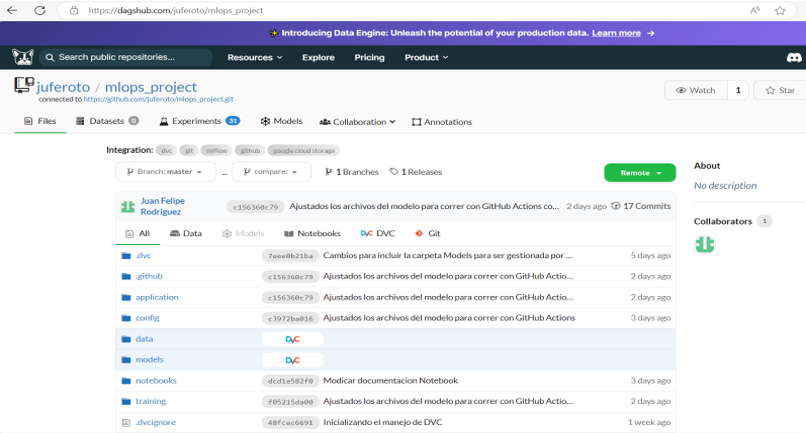
\includegraphics[width=0.6\textwidth]{resultados/herramientaDagshub.png}
\caption*{\footnotesize Fuente: Elaboración propia}
\label{fig:figuraHerramientaDagshub}
\end{figure}

Al acceder a la interfaz de DagsHub mediante el enlace detallado\footnote{El acceso al DagsHub del proyecto se encuentra \href{https://dagshub.com/juferoto/mlops_project}{aquí}.}, se inicia el proceso para utilizar esta plataforma. Para dar inicio a su uso, es posible crear una cuenta de forma gratuita. Esta suscripción no conlleva ningún costo y permite gestionar proyectos públicos sin restricciones. El límite máximo para el espacio de almacenamiento es de 100 gigabytes, proporcionando así un entorno accesible y eficiente para el manejo de datos en proyectos específicos.

La configuración del proyecto sigue la misma estructura que se detalló en el objetivo 3, tal como se describe en la figura \ref{fig:figuraHerramientaDagshub}. Al crear una cuenta en DagsHub, esta se vincula automáticamente con la cuenta Github utilizada para el versionado del código. Posteriormente, al compartir el enlace, se posibilita a otros usuarios acceder a la configuración del proyecto de manera sencilla. Este enfoque facilita la colaboración y el intercambio de información entre los miembros del equipo alineando la integración del proyecto de manera eficiente.

Cuando se busca incorporar almacenamiento externo, se presentan dos opciones específicas: AWS (Amazon S3) y Google Cloud (Google Storage). En este proyecto en particular, se optó por utilizar Google Cloud Storage (ver figura \ref{fig:figuraOpcionesAlmacena}). Al hacer clic en la opción correspondiente, se despliegan las configuraciones necesarias, permitiendo así realizar las acciones pertinentes para integrar y agregar el almacenamiento en la nube de Google al proyecto. Este proceso se simplifica mediante una interfaz intuitiva que guía al usuario a través de las opciones necesarias para una configuración eficaz.

\newpage

\begin{figure}[h]
\centering
\caption{Opciones para configurar un almacén de datos en DagsHub}
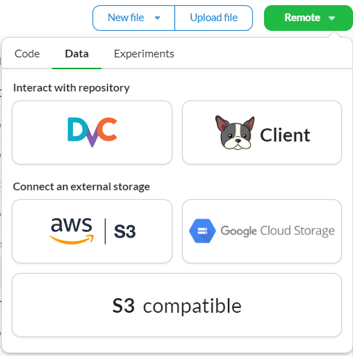
\includegraphics[width=0.4\textwidth]{resultados/opcionesAlmacena.png}
\caption*{\footnotesize Fuente: Elaboración propia}
\label{fig:figuraOpcionesAlmacena}
\end{figure}

Al seleccionar la opción ``Remote’’, se habilita la capacidad de visualizar los experimentos realizados con MLFlow (ver figura \ref{fig:figuraOpcionesMLFlow}). Es importante destacar que, en este contexto, la visualización no ocurre a nivel local, sino que se realiza de forma remota a través de la plataforma proporcionada por DagsHub con la “Go to mlflow UI”. Esto implica que los datos y resultados almacenados en MLFlow se encuentran accesibles de manera remota, gracias a la integración facilitada por DagsHub.

Para contextualizar y entender cómo se integra MLFlow en la nube con DagsHub, es esencial considerar los ajustes necesarios en el archivo principal ``main.yaml’’ de configuraciones. Al hacer la comparación, se identifica que en la configuración de MLFlow para trabajar en la nube, se requiere la adición de la URL que indica la ubicación específica del proyecto proporcionado por DagsHub, como el usuario y contraseña que provee DagsHub. Estos ajustes permiten que el proyecto se conecte con los recursos en la nube de MLFlow, facilitando así la gestión y visualización remota de experimentos y datos asociados con el proyecto realizado.

\newpage

\begin{figure}[h]
	\centering
	\caption{Opciones para usar remotamente MLFlow}
	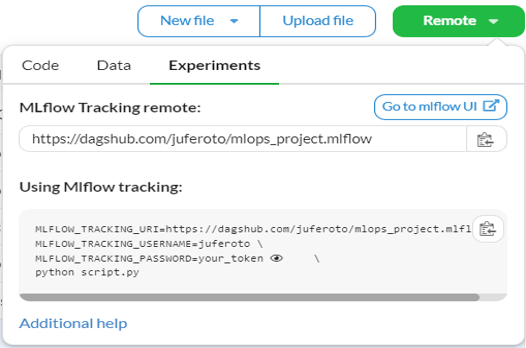
\includegraphics[width=0.6\textwidth]{resultados/opcionesMLFlow.png}
	\caption*{\footnotesize Fuente: Elaboración propia}
	\label{fig:figuraOpcionesMLFlow}
\end{figure}

\begin{figure}[h]
\centering
\caption{Configuración remota del MLFlow en el archivo ``main.yaml''}
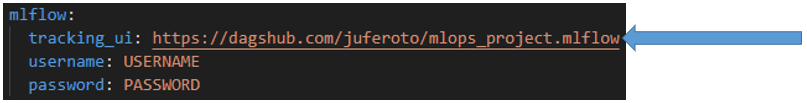
\includegraphics[width=1\textwidth]{resultados/confRemotaMLFlow.png}
\caption*{\footnotesize Fuente: Elaboración propia}
\label{fig:figuraConfRemotaMLFlow}
\end{figure}

El enlace específico del proyecto que provee DagsHub para MLflow es \\ \href{https://dagshub.com/juferoto/mlops_project.mlflow}{https://dagshub.com/juferoto/mlops\_project.mlflow}. Este enlace es el que se debe sustituir en el archivo correspondiente\footnote{Dentro del video se demuestra la gestión remota de la herramienta MLflow, siguiendo un proceso similar al realizado localmente. La diferencia clave radica en que esta vez se realiza de manera remota. El enlace para acceder al video se encuentra disponible para su visualización en YouTube \href{https://youtu.be/U2DqNOixHWw?si=OrJcIFpGiqfodAQy}{aquí}.}, tal como se señala en la imagen anterior.

Siguiendo con el despliegue en la nube, con el objetivo de asegurar un funcionamiento sin contratiempos tanto para la aplicación como para la API, es crucial determinar las dependencias necesarias. Por esta razón, se genera un archivo llamado requirements.txt., Este archivo se crea para enumerar todas las dependencias esenciales. 

\newpage

La instalación de estas dependencias se lleva a cabo mediante el comando 
\begin{verbatim}
pip install -r requirements.txt
\end{verbatim} 

Este proceso garantiza que todas las herramientas y dependencias necesarias se instalen de manera coherente, proporcionando así las condiciones apropiadas para el correcto funcionamiento de la aplicación y la API en la nube.

\begin{figure}[h]
	\centering
	\caption{Dependencias para trabajar con el proyecto localmente}
	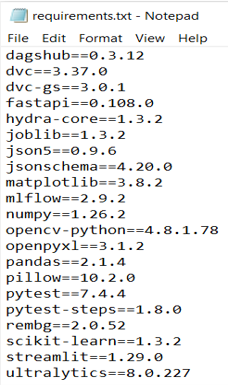
\includegraphics[width=0.3\textwidth]{resultados/dependenciasRemotas.png}
	\caption*{\footnotesize Fuente: Elaboración propia}
	\label{fig:figuraDependenciasRemotas}
\end{figure}

Para desplegar la aplicación y hacerla accesible en línea, una opción destacada es el uso de contenedores. Estos, según su descripción, son una tecnología de virtualización a nivel del sistema operativo que posibilita empacar y distribuir aplicaciones junto con sus dependencias y configuraciones.

La utilización de contenedores, especialmente a través de la conocida herramienta Docker, simplifica significativamente el proceso de desarrollo, implementación y gestión de aplicaciones. Docker se ha consolidado como una de las soluciones más utilizadas en este ámbito, ofreciendo una solución eficiente y coherente para el empaquetado, distribución y ejecución de aplicaciones \citep{orovengua2016}.

\newpage


\begin{figure}[h]
	\centering
	\caption{Diversas maneras de despliegue}
	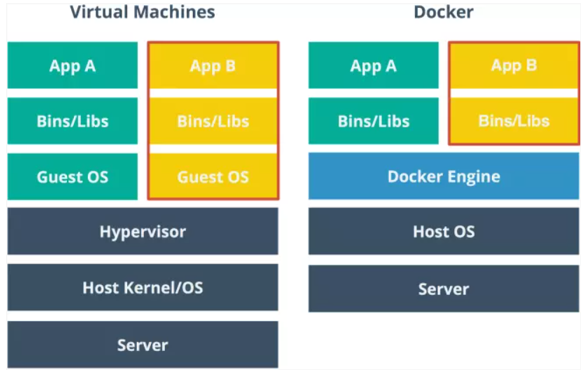
\includegraphics[width=0.8\textwidth]{resultados/diversosDespliegues.png}
	\caption*{\footnotesize Fuente: \cite{orovengua2016}}
	\label{fig:figuraDiversosDespliegues}
\end{figure}

Continuando con lo planteado por \cite{orovengua2016}, existen diversas maneras de llevar a cabo despliegues en entornos de nube, siendo dos de ellas notables: el uso de máquinas virtuales y la implementación de contenedores con Docker. La distinción clave entre ambas radica en que, mientras cada aplicación en máquinas virtuales requiere un sistema operativo virtualizado en su totalidad (utilizando, por ejemplo, un gigabyte de memoria RAM), los contenedores de Docker optimizan el rendimiento al aprovechar el kernel, es decir, el núcleo de la máquina real. Estos contenedores únicamente cargan en la memoria las bibliotecas o dependencias necesarias para ejecutar la aplicación, evitando la duplicación de recursos. Esto resulta en una eficiencia considerable, ocupando solo alrededor del 20\% del espacio en comparación con una máquina virtual de 1 gigabyte o 1024 megabytes. En este caso, el contenedor utiliza solo 200 megabytes de capacidad, ofreciendo así una solución más eficaz y económica en términos de recursos.

\newpage

Para emplear Docker se requiere de un archivo esencial en el contexto del uso de contenedores. Cabe destacar que, al optar por emplear contenedores con Docker, se requiere la creación de un archivo denominado Dockerfile\footnote{El código del archivo Dockerfile para la API se encuentra en GitHub \href{https://github.com/juferoto/mlops_project/tree/master/application/src}{aquí}.}. En este archivo se incorporan las configuraciones necesarias para el despliegue de una aplicación.


\begin{figure}[h]
	\centering
	\caption{Configuración del archivo Dockerfile para desplegar la API con FastAPI y Docker}
	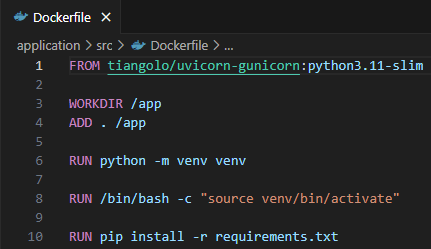
\includegraphics[width=0.8\textwidth]{resultados/configAPIDocker.png}
	\caption*{\footnotesize Fuente: Elaboración propia}
	\label{fig:figuraConfigAPIDocker}
\end{figure}

El código que se presenta en la imagen (ver figura \ref{fig:figuraConfigAPIDocker}) tiene como propósito desplegar la API. En este fragmento, se especifica la descarga de la versión necesaria de Python y de Uvicorn, que se utiliza para habilitar FastAPI, la cual expone la API para su acceso desde internet.

Adicionalmente, el código también detalla la carpeta de destino donde se copiará la aplicación. Se establece la creación de un entorno virtual, su activación, y la instalación de las dependencias necesarias para ejecutar la API de manera efectiva. \newline

Un archivo Dockerfile también es esencial para el despliegue de la aplicación. Mientras el Dockerfile previo estaba diseñado para desplegar la API, este nuevo archivo está destinado a implementar la aplicación con Streamlit, una herramienta que simplifica la creación de la aplicación en general\footnote{El código del archivo Dockerfile para la aplicación se encuentra en GitHub \href{https://github.com/juferoto/mlops_project/tree/master/application/src/webapp}{aquí}}.

\newpage

\begin{figure}[h]
	\centering
	\caption{Configuración del archivo Dockerfile para desplegar la aplicación con Streamlit y Docker}
	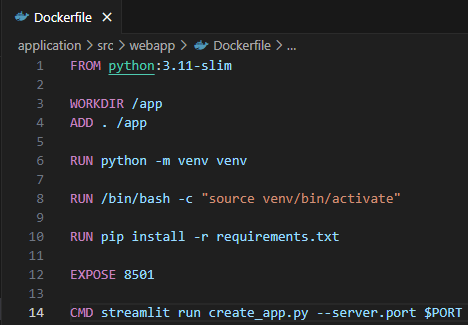
\includegraphics[width=0.8\textwidth]{resultados/configAplicacionDocker.png}
	\caption*{\footnotesize Fuente: Elaboración propia}
	\label{fig:figuraConfigAplicacionDocker}
\end{figure}

En este contexto, se vuelve a crear el archivo Dockerfile, especificando la imagen necesaria de Python. Se detalla la carpeta de destino donde se copiará el proyecto. El proceso implica la creación y activación de un entorno virtual específico, la instalación de dependencias cruciales, la exposición del puerto designado para acceder a la aplicación, y la ejecución de un comando que permite visualizar la aplicación desde internet. \newline

Para lograr lo anterior, es necesario emplear contenedores como medio de empaquetamiento y almacenamiento de toda la información necesaria. Una vez que se haya encapsulado la información dentro de un contenedor, el siguiente paso implica transferir dicho contenedor a una herramienta o proveedor de servicios en la nube para facilitar el despliegue. En este caso, como se detalló en el tercer objetivo, se optó por utilizar Google Cloud Platform (GCP) como proveedor de servicios en la nube. \newline

\newpage

GCP ofrece una amplia gama de servicios y herramientas que abarcan desde plataformas complejas hasta infraestructuras personalizables. Esta diversidad brinda a los desarrolladores la flexibilidad de seleccionar la solución que mejor se ajuste a sus necesidades específicas. En el contexto de este proyecto en particular, se eligieron tres servicios de GCP que se consideran más idóneos para satisfacer los requisitos establecidos. Los servicios seleccionados para realizar despliegues con GCP en la nube para el proyecto son:

\begin{itemize}
	\item \textbf{Google Cloud Storage}: Se utiliza para el almacenamiento y recuperación de datos.
	\item \textbf{Google Artifact Registry}: Se usa para la gestión de artefactos (contenedores) de software del proyecto.
	\item \textbf{Google Cloud Run}: Se utiliza para desplegar y ejecutar los contenedores de manera administrada y escalable.
\end{itemize}

La selección de estos servicios fue posible gracias a la extensa variedad que GCP proporciona, permitiendo así una adaptación precisa a las demandas del proyecto. Estos servicios específicos se eligieron para garantizar una implementación correcta de la solución propuesta. Tanto Google Artifact Registry, como, Google Cloud Run fueron los que se usaron para la parte de los contenedores. \newline

Antes de poder aprovechar las opciones ofrecidas anteriormente, es necesario establecer configuraciones y accesos adecuados para hacer uso de sus servicios. Este proceso es aplicable a los tres componentes esenciales de Google que se emplearon (ver anexo \href{https://drive.google.com/file/d/1DbWHxnWBgaB8Tp3J8hLYelR91bEdglr-/view?usp=drive_link}{1}). \newline

Las URLs que genera Cloud Run son usualmente estáticas por cada contenedor a desplegar. En ese sentido, la URL para hacer uso de la API es \href{https://api-plague-predict-6gzk55suba-uc.a.run.app/docs}{https://api-plague-predict-6gzk55suba-uc.a.run.app/docs} y la URL para hacer uso de la aplicación es \href{https://web-plague-predict-6gzk55suba-uc.a.run.app}{https://web-plague-predict-6gzk55suba-uc.a.run.app}. Para hacer uso de estas, se debe contar previamente a que los contenedores se hayan creado y desplegado correctamente. \newline

A continuación, se presenta en un video como se ve la API y la aplicación en la nube, con el modelo que ha sido seleccionado mediante MLFlow y se ha marcado para estar en producción\footnote{El video correspondiente a este proceso está disponible en YouTube \href{https://youtu.be/GV5-WZFxAOU?si=juse0Gmu4mX00cAJ}{aquí}}.

\newpage

\subsubsection{Monitoreo sobre el modelo}

Continuando con el tema, centrémonos ahora en la herramienta que simplifica los despliegues de la aplicación y la API de manera automatizada. La necesidad de esta herramienta radica en lo tedioso que implicaría realizar estos despliegues manualmente. En un enfoque manual, se tendría que crear el contenedor, enviarlo a la nube y, posteriormente, especificar la imagen que debe utilizar Google Cloud Run una vez que el contenedor ha sido guardo en el registro (Artifact Registry). Luego, sería necesario obtener la URL para su uso. Este proceso, aunque posible de realizar manualmente, se vuelve más eficiente y menos propenso a errores al utilizar GitHub Actions, una herramienta de automatización integrada con GitHub. \newline

GitHub Actions es un servicio que permite a los ingenieros de software automatizar diversas tareas en respuesta a eventos específicos dentro del repositorio. En el contexto del proyecto, las tareas se configuran mediante flujos de trabajo definidos en archivos YAML. Estos flujos de trabajo simplifican la ejecución de pruebas, la construcción de la API y la aplicación, junto con los despliegues. GitHub Actions no solo facilita la automatización de estos procesos, sino que también respalda la integración continua y el despliegue continuo. \newline

Esta integración automatizada con GitHub Actions no solo agiliza el ciclo de desarrollo, sino que también asegura la coherencia y confiabilidad en el proceso de despliegue de la aplicación y la API. Con esta herramienta, se logra una gestión eficiente y automatizada de todo el ciclo de vida del modelo para llevarlo a producción, desde la integración de cambios hasta la entrega y despliegue en la infraestructura de Google Cloud Run. \newline

En el contexto específico del proyecto se han definido tres archivos clave: \\ validate\_deploy\_app.yaml, validate\_model.yaml y validate\_model\_automatically.yaml. Cada uno de estos archivos desempeña un papel en la validación del modelo y despliegue de la API y la aplicación como esta descrito en la figura \ref{fig:figuraEstructuraCodValidate}. 


\newpage

\begin{figure}[h]
	\centering
	\caption{Estructura del archivo validate\_deploy\_app.yaml}
	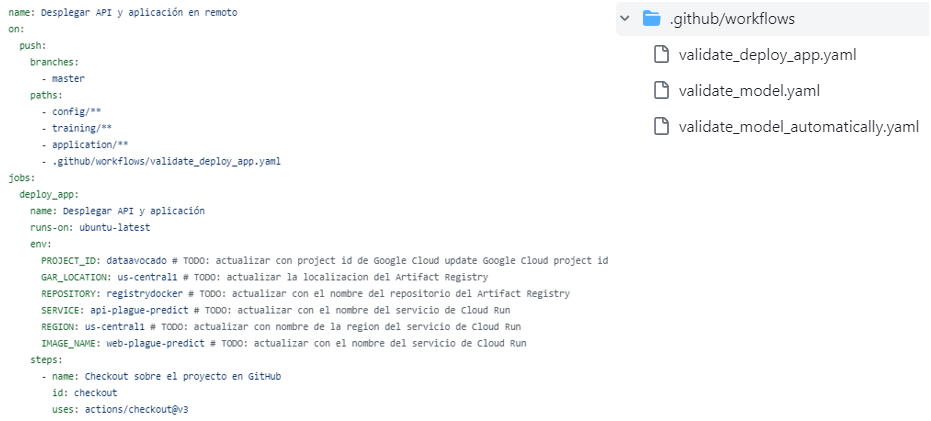
\includegraphics[width=1\textwidth]{resultados/estructuraCodValidate.png}
	\caption*{\footnotesize Fuente: Elaboración propia}
	\label{fig:figuraEstructuraCodValidate}
\end{figure}

En particular, el archivo validate\_deploy\_app.yaml tiene la responsabilidad de gestionar la validación del despliegue de la aplicación. Este proceso es esencial para garantizar que la aplicación se despliegue de manera correcta y coherente en el entorno de Google Cloud Run\footnote{La estructura completa y detallada de cada uno de estos archivos se encuentra disponible en el enlace proporcionado, ofreciendo una visión profunda de cómo se gestionan las validaciones y despliegues en el marco del proyecto de ingeniería de datos. El código se encuentra en GitHub \href{https://github.com/juferoto/mlops_project/tree/master/.github/workflows}{aquí}}. \newline

Dentro de GitHub Actions, la estructura se organiza en ``Jobs'', cada uno de los cuales contiene pasos específicos a seguir. En este caso particular, se ilustrará el contenido del workflow llamado ``Desplegar API y aplicación en remoto''. \newline

El ``Job'' que es responsable de desplegar la API y la aplicación, se inicia con la denominación general del archivo. En este contexto, se identifica como ``Desplegar API y aplicación''. Dentro de este Job, se definen varios pasos, y el primero de ellos es la acción de ``Checkout'', que básicamente implica obtener la totalidad del proyecto almacenado en GitHub. La finalidad de este paso inicial es asegurar que el entorno de ejecución cuente con la versión más reciente y completa del proyecto antes de proceder con las tareas de despliegue de la API y la aplicación.

\newpage

\begin{figure}[h]
	\centering
	\caption{Continuidad de la estructura del archivo validate\_deploy\_app.yaml}
	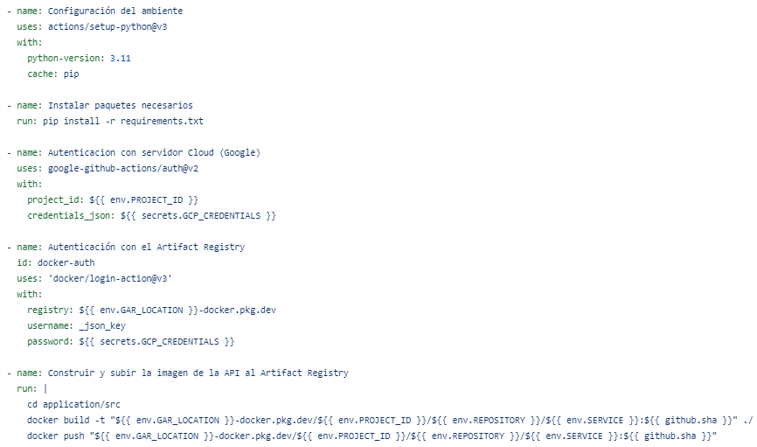
\includegraphics[width=1\textwidth]{resultados/estructuraCodValidate2.png}
	\caption*{\footnotesize Fuente: Elaboración propia}
	\label{fig:figuraEstructuraCodValidate2}
\end{figure}

Continuando con el análisis del archivo, se incorpora otro paso fundamental: la configuración del ambiente (ver figura \ref{fig:figuraEstructuraCodValidate2}). En este caso, se solicita cargar una versión específica de Python, en este ejemplo, la versión 3.11. Además, se lleva a cabo la instalación de los paquetes necesarios. Este paso es crucial para preparar el ambiente con las herramientas y dependencias adecuadas que se han mencionado anteriormente. La selección y configuración de la versión de Python es esencial para garantizar la compatibilidad con la aplicación y la API que se desplegarán. \newline

Para llevar a cabo el despliegue en la nube, es imprescindible contar con el archivo Dockerfile. Se recuerda que este archivo corresponde tanto para el despliegue de la API y la aplicación. Este paso asegura que los elementos necesarios estén presentes y correctamente configurados para la implementación en cloud.

\newpage

La autenticación se convierte en otro componente esencial de este proceso. El archivo se autentica tanto con el servidor de GCP como con su componente Artifact Registry, que es la ubicación donde se almacenan los contenedores. Esta autenticación es necesaria para garantizar la autorización adecuadas al interactuar con los servicios de Google Cloud, y especialmente con el lugar donde residen las imágenes de los contenedores.

Posteriormente, el proceso implica la construcción y la carga de la imagen. Es decir, se toma el archivo Docker previamente configurado y se genera la imagen correspondiente. Esta imagen se sube al Artifact Registry mencionado anteriormente. Este paso final es para asegurar que la imagen esté disponible y lista para el despliegue en Google Cloud Run.

\begin{figure}[h]
	\centering
	\caption{Despliegue de la API y aplicación a Google Cloud Run}
	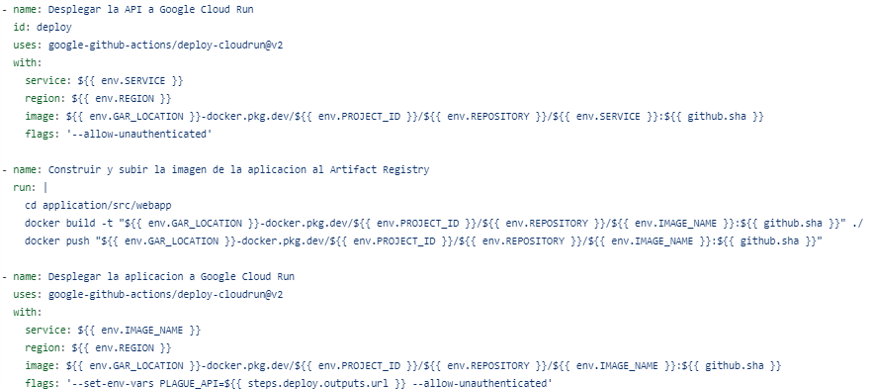
\includegraphics[width=1\textwidth]{resultados/estructuraCodValidate3.png}
	\caption*{\footnotesize Fuente: Elaboración propia}
	\label{fig:figuraEstructuraCodValidate3}
\end{figure}

Al realizar el despliegue de la API, llevamos a cabo una serie de pasos específicos. En primer lugar, se procede a construir y subir la imagen al Artifact Registry. En segundo lugar, se ejecuta un paso adicional para desplegar la aplicación en Google Cloud. Tanto para la API como para la aplicación en sí, es esencial seguir cuidadosamente los comandos establecidos, garantizando así la disponibilidad y la integridad tanto de la API como de la aplicación.

\newpage

Aquí se presentan configuraciones basadas en la documentación oficial de GitHub para llevar a cabo el despliegue en GitHub Actions. Estas configuraciones se ajustan a las prácticas recomendadas por GitHub para la implementación de flujos de trabajo automatizados. \newline

Estas configuraciones, extraídas directamente de la documentación oficial, proporcionan una base sólida para la ejecución eficiente de acciones en GitHub. Al seguir estas directrices, se asegura la coherencia y la conformidad con las prácticas recomendadas. \newline

Cabe señalar que, el archivo anterior validate\_deploy\_app.yaml se activa automáticamente cada vez que se realiza un ``Push'', es decir, cuando se modifica el algoritmo del modelo o alguna de las partes del proyecto. Este escenario puede surgir debido a la identificación de nuevas adiciones o ajustes de parámetros esenciales. En situaciones donde el modelo almacenado en la nube no coincide con el correcto, es necesario realizar un nuevo entrenamiento y generar una versión actualizada. Este proceso de reentrenamiento también implica que el código subyacente ha experimentado modificaciones. \newline

Además, este desencadenante automático también ocurre cuando se manipulan datos que se deben cargar. En tal caso, se realiza un ``Push'' hacia la rama principal, que en este contexto es la rama Master en GitHub. \newline

Este enfoque automatizado garantiza que cualquier cambio en el código del modelo o en los datos sea detectado y desencadene el proceso de validación. La ejecución del flujo de trabajo de GitHub Actions asegura la consistencia, la actualización del modelo y el despliegue del mismo en un entorno local, manteniendo la coherencia entre el código, los datos y la implementación realizada. \newline

Para validar el modelo y la aplicación, se emplea un enfoque similar en GitHub Actions, donde se define un workflow con el nombre ``Validar modelo y aplicación en local'', este archivo contiene distintos ``Jobs'', cada uno con sus respectivos pasos detallados para llevar a cabo la validación (ver figura \ref{fig:figuraEstructuraCodValidateModel}). 

\newpage

Cuando se trata de validar el proyecto en el contexto de Git, ya no se realiza directamente en la rama Master. En su lugar, se adopta un enfoque más colaborativo, donde la validación se lleva a cabo al crear una nueva rama. Esta práctica busca asegurar la integridad de los datos y la calidad del modelo antes de incorporarlo a la rama principal. \newline

La validación sobre el modelo y la aplicación se realiza mediante un pull request, este paso adicional se implementa con el propósito de evaluar el estado en que se encuentren los datos, el desempeño del modelo y el despliegue de la aplicación en local, antes de fusionarse con la rama principal. Esta estrategia es relevante en entornos de trabajo colaborativo, donde distintas personas pueden estar modificando diferentes secciones del proyecto. \newline

La incorporación de Pull requests permite a los científicos de datos validar de manera individual cómo se comporta su modelo con nuevos datos o cambios específicos. Esta práctica facilita la detección temprana de posibles problemas y proporciona una oportunidad para ajustar y mejorar antes de fusionar los cambios en la rama principal. \newline

En ese sentido, en el contexto de la validación del modelo (ver figura \ref{fig:figuraEstructuraCodValidateModel}), se detalla el procedimiento para evaluar el comportamiento del modelo antes de fusionarlo con la rama principal. En este escenario, se crea una rama auxiliar para la validación. Se inicia un Pull request en esta rama para observar cómo se comporta el proyecto con nuevos datos o cambios específicos. Si la evaluación resulta satisfactoria y todos los aspectos son adecuados, entonces el científico de datos puede proceder a fusionar los cambios con la rama principal. 

\newpage

\begin{figure}[h]
	\centering
	\caption{Estructura del archivo validate\_model.yaml}
	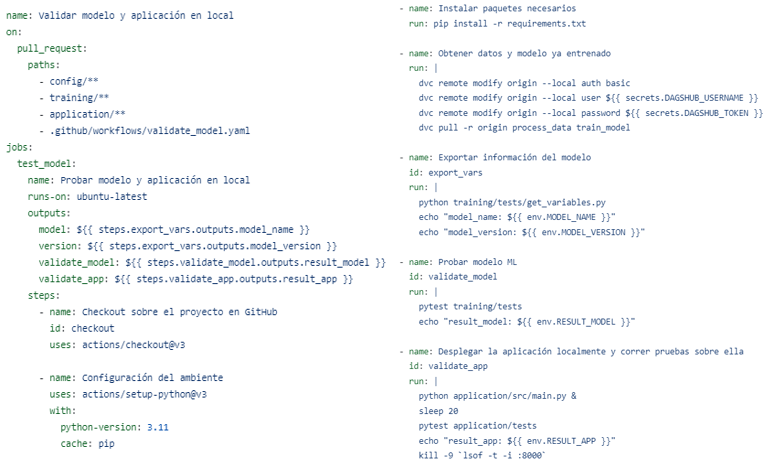
\includegraphics[width=0.7\textwidth]{resultados/estructuraCodValidateModel.png}
	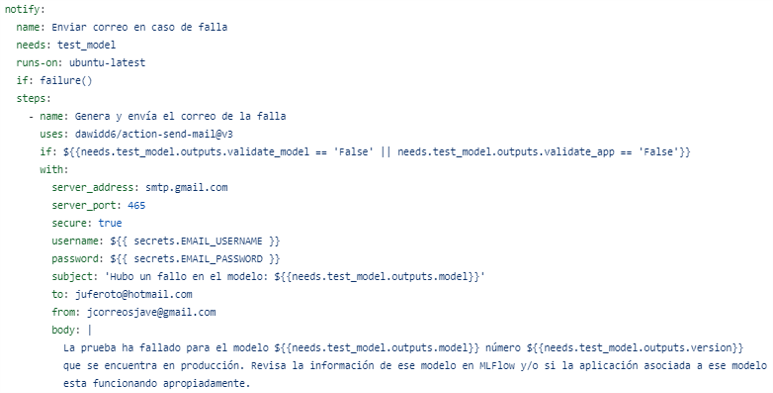
\includegraphics[width=0.7\textwidth]{resultados/estructuraCodValidateModel2.png}
	\caption*{\footnotesize Fuente: Elaboración propia}
	\label{fig:figuraEstructuraCodValidateModel}
\end{figure}

\newpage

El último archivo, denominado validate\_model\_automatically.yaml, ha sido creado con la finalidad de ejecutar periódicamente un workflow específico llamado ``Validar modelo y aplicación automáticamente''.

\begin{figure}[h]
	\centering
	\caption{Estructura del archivo validate\_model\_automatically.yaml}
	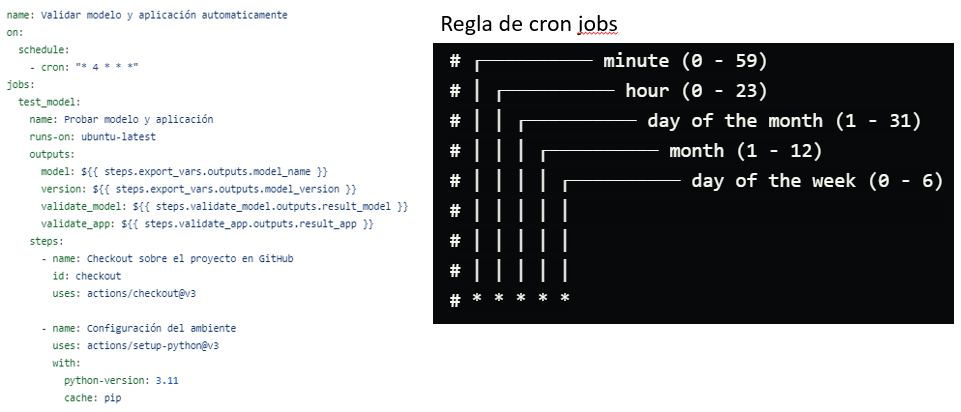
\includegraphics[width=0.7\textwidth]{resultados/estructuraCodValidateAuto.png}
	\caption*{\footnotesize Fuente: Elaboración propia}
	\label{fig:figuraEstructuraCodValidateAuto}
\end{figure}

El workflow se ejecuta de manera automática según una programación establecida mediante un cron. Los cron son convenciones para tareas programadas, donde los campos indican, en orden, minutos, horas, mes y día de la semana. En este caso particular, se ha definido que la tarea programada se ejecute todos los días a las 4 de la mañana. Se ha seleccionado este horario considerando que no todas las personas estarán conectadas o disponibles a esa hora, lo cual optimiza la ejecución automática y periódica del workflow. \newline

Es importante señalar que este archivo se centra en realizar pruebas tanto al modelo como al despliegue de la aplicación como se muestra en la figura \ref{fig:figuraEstructuraCodValidateAutoDet}. La secuencia de pasos establecidos en este archivo asegura la ejecución efectiva de estas pruebas automáticas de manera programada.

\newpage

\begin{figure}[h]
	\centering
	\caption{Continuidad de la estructura del archivo validate\_model\_automatically.yaml}
	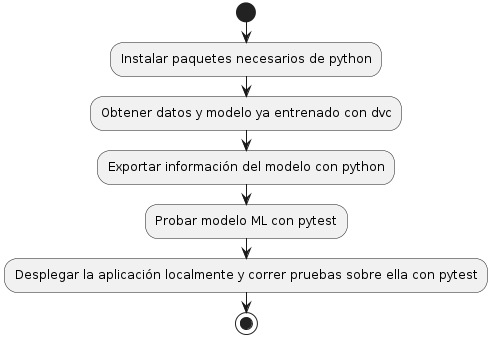
\includegraphics[width=0.8\textwidth]{resultados/estructuraCodValidateAutoDet.png}
	\caption*{\footnotesize Fuente: Elaboración propia}
	\label{fig:figuraEstructuraCodValidateAutoDet}
\end{figure}

Para detectar un fallo durante la ejecución de las pruebas, ya sea al evaluar el modelo o al intentar desplegar la aplicación localmente, se han establecido las pruebas utilizando pytest. En caso de que alguna de estas pruebas falle, se activa otro ``Job'' denominado ``Enviar correo en caso de falla'' (ver figura \ref{fig:figuraEstructuraCodValidateAutoNot}). Este ``Job'' tiene la función de notificar sobre la detección de un fallo en alguna de las dos tareas.

\begin{figure}[h]
	\centering
	\caption{Estructura de notificación de fallo del archivo validate\_model\_automatically.yaml}
	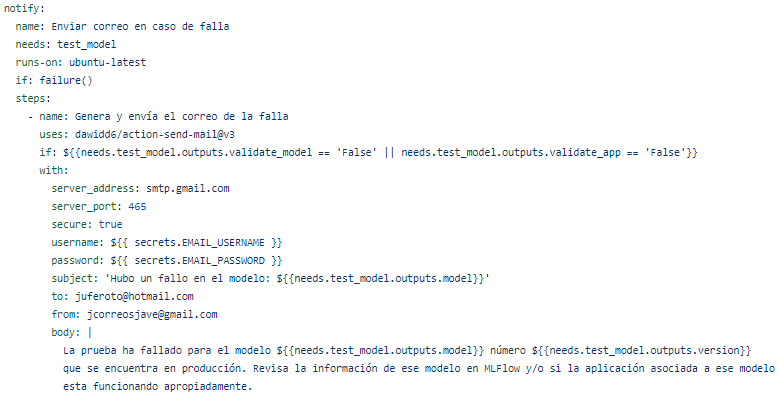
\includegraphics[width=0.7\textwidth]{resultados/estructuraCodValidateAutoNot.png}
	\caption*{\footnotesize Fuente: Elaboración propia}
	\label{fig:figuraEstructuraCodValidateAutoNot}
\end{figure}

\newpage

La implementación de las pruebas en pytest ofrece una evaluación específica para identificar cualquier inconveniente tanto en el modelo como en el despliegue de la aplicación. La activación del ``Job'' sirve como mecanismo de alerta temprana, proporcionando la información necesaria en el caso de que alguna de las tareas no se ejecute conforme a lo esperado\footnote{Se manda a ejecutar periódicamente un workflow de Github Actions que reevalúa el desempeño del modelo y envía un correo electrónico en caso de contar con un valor inferior predefinido. Esto se envía a la persona a cargo del modelo para que lo verifique, y después ejecute un despliegue con el modelo que considere está en buenas condiciones, para ser usado desde la API y aplicación.}, situación que es enviada a un correo electrónico especificando el nombre y el número del modelo que se encuentra en producción.

\begin{figure}[h]
	\centering
	\caption{Estructura del correo recibido}
	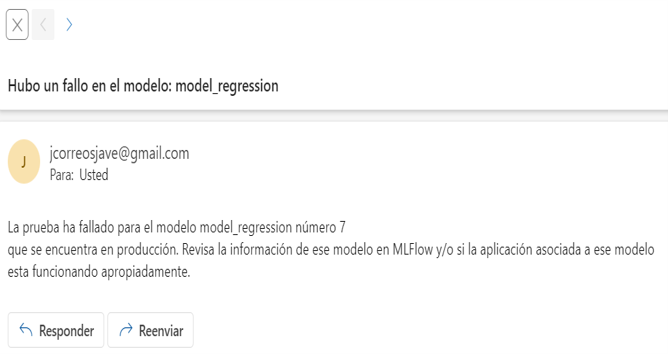
\includegraphics[width=0.9\textwidth]{resultados/estructuraCorreoRecibido.png}
	\caption*{\footnotesize Fuente: Elaboración propia}
	\label{fig:figuraEstructuraCorreoRecibido}
\end{figure}


Como se viene señalando, las pruebas se desarrollaron con pytest, siendo éste una dependencia de Python. La prueba con Pytest al momento de evaluar el modelo, verifica 3 métricas (accuracy, precision y recall) establecidas a un valor del 70\%, en donde si se cuenta con valores inferiores en una de las tres, se envía una alerta al científico de datos (por correo), para que así proceda a revisar el estado del modelo. Esto se hace ejecutando una tarea programada diaria, que es ejecutada cada día a las 4 am usando GitHub Actions. 

\newpage

Aquí se presenta la estructura de los archivos que se emplearon específicamente para realizar la evaluación del desempeño del modelo\footnote{El código para evaluar el desempeño del modelo se encuentra en GitHub \href{https://github.com/juferoto/mlops_project/tree/master/training/tests}{aquí}}. Entre ellos, se destaca un archivo llamado ``get\_variables.py'', cuya finalidad es obtener variables necesarias para el proceso, siendo utilizado en GitHub Actions. Este archivo proporciona información como el nombre del modelo y la versión del modelo, que se utilizarán en caso de fallas en las pruebas de rendimiento del modelo y despliegue.


\begin{figure}[h]
	\centering
	\caption{Estructura carpeta tests del modelo y estructura del archivo get\_variables.py}
	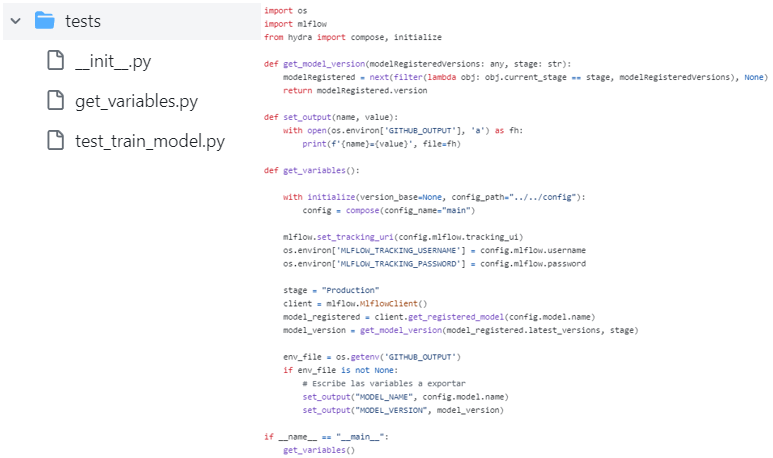
\includegraphics[width=0.8\textwidth]{resultados/estructuraCarTestGet.png}
	\caption*{\footnotesize Fuente: Elaboración propia}
	\label{fig:figuraEstructuraCarTestGet}
\end{figure}

Esta organización de archivos refleja una estrategia bien definida para evaluar el desempeño del modelo en el contexto de la ciencia de datos e ingeniería de software. La modularidad y la claridad en la estructura facilitan la gestión y ejecución efectiva de las pruebas, contribuyendo a un proceso adecuado.

Además, el archivo principal para evaluar el rendimiento del modelo se realiza una funcionalidad clave. En este documento, se obtiene el modelo de MLFlow, que representa la versión actualmente en producción. Asimismo, se accede a los conjuntos de datos de prueba, y finalmente, se realiza la prueba de rendimiento, utilizando el modelo de regresión logística (ver figura \ref{fig:figuraEstructuraCodTestTrain}).

\newpage

\begin{figure}[h]
	\centering
	\caption{Estructura del archivo test\_train\_model.py}
	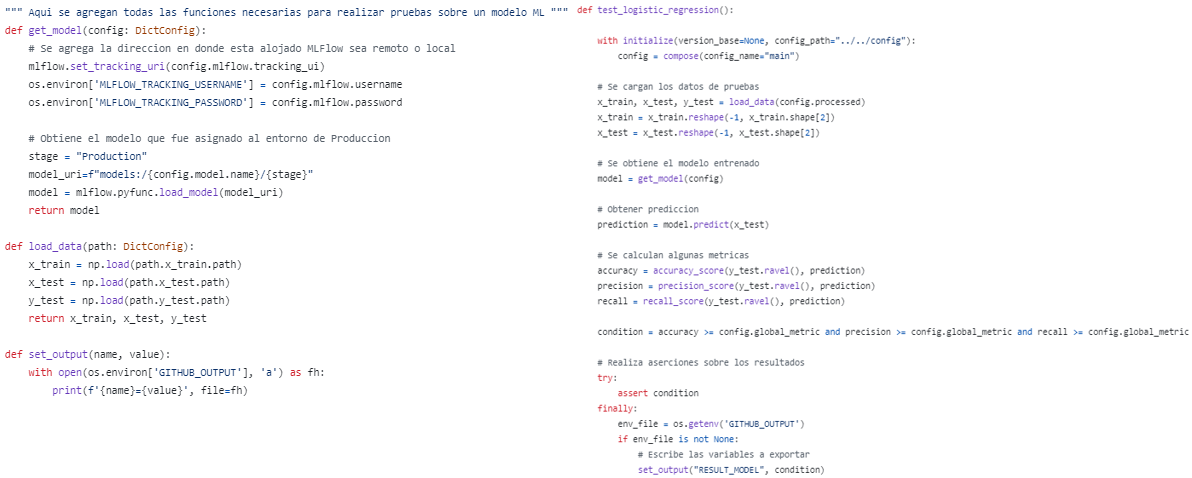
\includegraphics[width=1\textwidth]{resultados/estructuraCodTestTrain.png}
	\caption*{\footnotesize Fuente: Elaboración propia}
	\label{fig:figuraEstructuraCodTestTrain}
\end{figure}

La obtención del modelo de MLFlow es un paso crítico, ya que garantiza que se esté evaluando la versión en producción, asegurando consistencia en el proceso de evaluación de rendimiento.

Adicionalmente, después de obtener las predicciones con el modelo obtenido desde MLFlow, se procede a calcular diversas métricas de evaluación. Estas métricas incluyen, entre otras, la exactitud (accuracy), la precisión (precision) y la sensibilidad (recall).

Este proceso inicia con la obtención de las predicciones a partir del modelo adquirido. Posteriormente, se realizan cálculos precisos para evaluar el rendimiento del modelo. Las métricas específicas mencionadas, como accuracy, precision y recall, proporcionan una visión del comportamiento del modelo en función de sus predicciones.

Asimismo, Se compara con la variable que representa la métrica global previamente mencionada y se establece en un valor objetivo del 0.7 o 70\%. Esta variable actúa como un umbral de referencia, proporcionando un criterio claro para la evaluación del rendimiento del modelo. Al establecerla en 0.7, se indica un nivel deseado de desempeño en la salida del modelo.

\newpage

Para finalizar se muestra la evaluación del despliegue de la aplicación con la estructura del archivo test\_service.py para establecer el comportamiento del servicio:

\begin{figure}[h]
	\centering
	\caption{Evaluación del despliegue de la aplicación del archivo test\_service.py}
	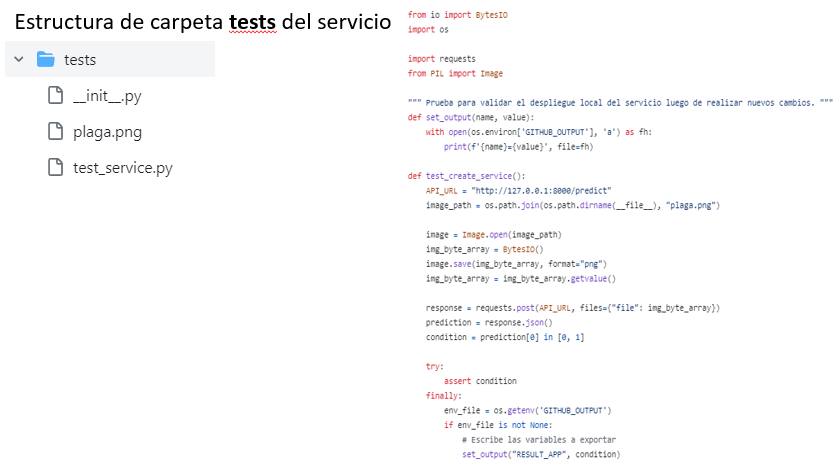
\includegraphics[width=0.8\textwidth]{resultados/estructuraCodTestService.png}
	\caption*{\footnotesize Fuente: Elaboración propia}
	\label{fig:figuraEstructuraCodTestService}
\end{figure}

Este código tiene como objetivo evaluar el comportamiento del servicio, indicando que la aplicación se ha ejecutado correctamente. La lógica implementada verifica si la API ha sido cargada exitosamente y si está generando los resultados esperados. La evaluación se basa en una condición, donde si la condición se cumple, se considera que la prueba ha sido exitosa\footnote{El código para evaluar el despliegue de la aplicación se encuentra en GitHub \href{https://github.com/juferoto/mlops_project/tree/master/application/tests}{aquí}}. En caso contrario, si la condición no se satisface, la prueba falla y se activa la notificación por correo electrónico.

El proceso de monitorear métricas y ajustar el modelo para reentrenamiento si es necesario y así evitar la degradación del modelo y mostrar nuevamente en la nube la API y aplicación con el nuevo modelo seleccionado, se evidencia desde el video preparado para su acceso\footnote{Se muestra la notificación recibida por correo, para luego monitorear el modelo y seleccionar uno distinto o realizar reentrenamiento, debido a que hubo una degradación del modelo. Además, se muestra nuevamente la API y aplicación en la nube con el nuevo modelo seleccionado, en el siguiente enlace: \href{https://youtu.be/U2DqNOixHWw}{https://youtu.be/U2DqNOixHWw}}.

